\documentclass[UTF8]{ctexart}
\usepackage{ctex}
\usepackage{geometry}
\geometry{left=3.18cm,right=3.18cm,top=2.54cm,bottom=2.54cm}
\usepackage{graphicx}
\usepackage{framed}
\usepackage{fancyhdr}
\usepackage{setspace}
\pagestyle{fancy}%清除原页眉页脚样式
\fancyhf{}
\fancyhead[C]{华中科技大学电信学院}
\fancyfoot[C]{\thepage}
% \pagestyle{plain}
\begin{document}
\begin{center}
    \quad \\
    \quad \\
    % \kaishu \fontsize{35}{5} \textbf{华 中 科 技 大 学}
    % \vskip 3cm
    \fangsong \fontsize{49}{5}《数字信号处理》 实验报告
    \vskip 3cm
    \heiti \zihao{1}\textbf{数字滤波器}
    \fangsong \zihao{1} 的设计实现与使用
\end{center}

\makeatletter
\newcommand\dlmu[2][4cm]{\hskip1pt\underline{\hb@xt@ #1{\hss#2\hss}}\hskip3pt}
\makeatother

\vskip 3cm
\begin{center}
    \zihao{3}
    \begin{tabular}{rl}
         & \makebox[4em][s]{学生姓名}	\hspace{0.2cm}	\dlmu[9cm]{赵展}
         \\
         & \makebox[4em][s]{学号}	\hspace{0.2cm}	\dlmu[9cm]{U202117282}
         \\
         & \makebox[4em][s]{专业班级}	\hspace{0.2cm}		\dlmu[9cm]{种子2101班}
         \\
         & \makebox[4em][s]{实验平台}	\hspace{0.2cm}		\dlmu[9cm]{Matlab R2023b on Windows}
         \\
         & \makebox[4em][s]{联系方式}	\hspace{0.2cm}		\dlmu[9cm]{15225929727}
         \\
    \end{tabular}
    \vskip 3cm
    2023年11月5日
\end{center}
\newpage
\tableofcontents
\newpage
\section{实验目的}
\begin{itemize}
    \item 掌握使用FFT进行信号谱分析的方法;
    \item 设计数字滤波器对指定的语音信号进行滤波处理。
\end{itemize}
\section{实验内容}
\begin{itemize}
    \item 使用Matlab的fft 函数对语音信号进行频谱分析,找出干扰信号的频谱;
    \item 设计数字滤波器滤除语音信号中的干扰分量,并进行播放对比。
\end{itemize}
\section{实验过程与结果分析}
\subsection{理想带阻滤波器}
对信号源函数进行傅里叶变换和频谱分析,然后设计理想带阻滤波器进行滤波。其中带阻滤波器的脚本函数如下:
\begin{verbatim}
    % band reject filter design
    function [afterfilter] = band_reject(audio_data, f, fs)
    w = 2 * pi * (f / fs);
    A =-2 * cos(w);
    h_n = [1, A, 1];
    afterfilter = conv(audio_data, h_n);
\end{verbatim}
该滤波器令$|H{e^{j\omega}}|=0$可以求出$A=-2\cos(\omega)$,在时域上卷积计算就可以将特殊的噪音部分的波滤掉。
首先将原信号波进行频谱分析,在matlab中输入以下代码,到如图\ref{img:1}所示的结果
\begin{verbatim}
    % read original audio wave
    clear all;
    close all;
    [audio_data, fs] = audioread('..\dsp_lab\lab2\SunshineSquare.wav');
    time = (length(audio_data)- 1) / fs; % get audio time
    n = 0 : length(audio_data)- 1;
    tt = 0 : 1 / fs : time; % generate time vector
    % freq domain frequency resolution
    freq_res = n * fs / length(audio_data);
    fft_audio_data = fft(audio_data); % do fft to audio_data
    subplot(2,1,1);
    plot(tt, audio_data);
    title('原始声音信号时域波形');
    subplot(2,1,2);
    plot(freq_res, abs(fft_audio_data)); % plot freqency domain data
    title('原始声音信号频域波形');
\end{verbatim}
\begin{figure}[htbp]
    \centering
    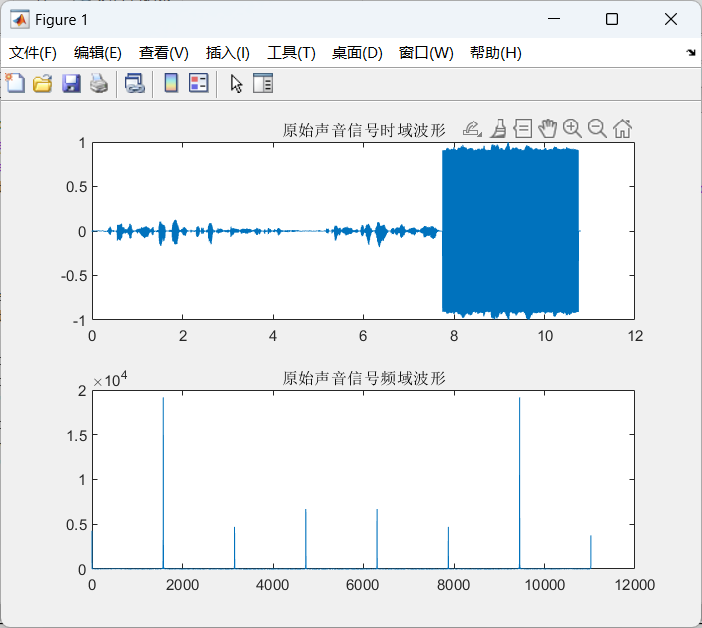
\includegraphics[width=0.6\textwidth]{1.png}
    \caption{原信号时域波形和频谱}
    \label{img:1}
\end{figure}
然后我先后进行了四次滤波处理,不断滤除噪声。
\paragraph{第一次滤波}~{}\par
第一次滤除0Hz左右的噪声,使用如下代码,得到如图\ref{img:2}所示的波形结果。
\begin{verbatim}
    % read original audio wave
    clear all;
    close all;
    [audio_data, fs] = audioread('..\dsp_lab\lab2\SunshineSquare.wav');
    time = (length(audio_data) -1)/ fs; % get audio time
    n = 0 : length(audio_data)- 1;
    tt = 0 : 1 / fs : time; % generate time vector
    % freq domain frequency resolution
    freq_res = n * fs / length(audio_data);
    audio_1 = band_reject(audio_data, 0, fs);
    audio_1 = audio_1(1 : end-2); % remove the last two elements.
    fft_audio_1 = fft(audio_1);
    subplot(2,1,1);
    plot(tt, audio_1);
    title('滤波一次后声音信号时域波形');
    subplot(2,1,2);
    plot(freq_res, abs(fft_audio_1));
    title('滤波一次后声音信号频域波形');
\end{verbatim}
\begin{figure}[htbp]
    \centering
    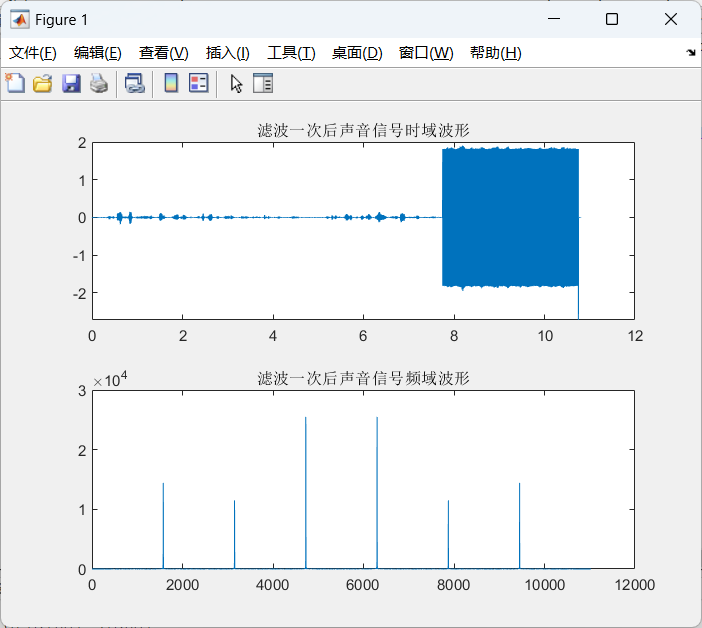
\includegraphics[width=0.6\textwidth]{2.png}
    \caption{第一次滤波后的时域频域信号}
    \label{img:2}
\end{figure}
\paragraph{第二、三次滤波}~{}\par
第二、三次滤除1574.99Hz、3149.97Hz左右的噪声,使用相似的代码,得到如图\ref{img:3},\ref{img:4}所示的波形结果。
\begin{figure}[htbp]
    \centering
    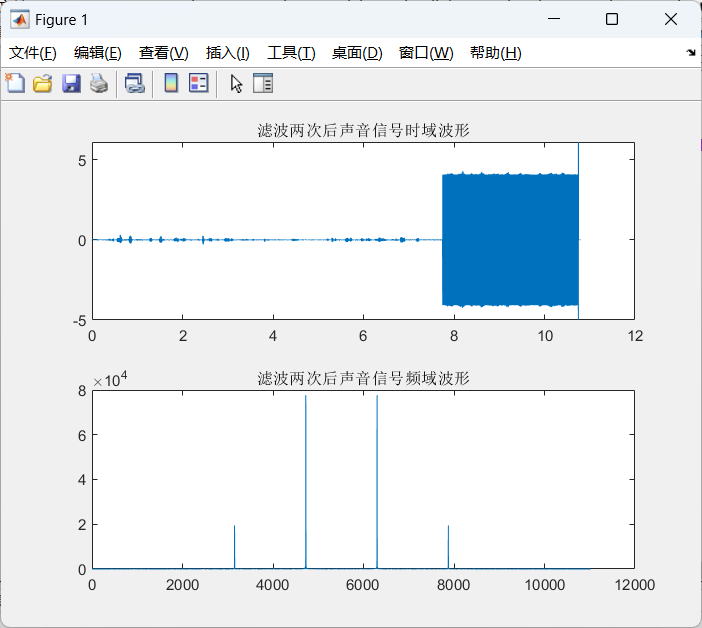
\includegraphics[width=0.6\textwidth]{3.png}
    \caption{第二次滤波后的时域频域信号}
    \label{img:3}
\end{figure}
\begin{figure}[htbp]
    \centering
    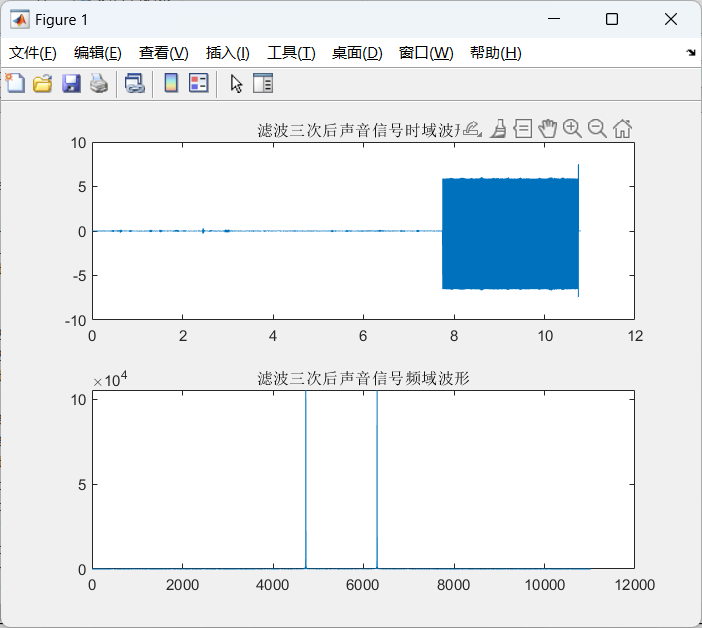
\includegraphics[width=0.6\textwidth]{4.png}
    \caption{第三次滤波后的时域频域信号}
    \label{img:4}
\end{figure}
\paragraph{第四次滤波}~{}\par
第四次滤除4724.96Hz左右的噪声,使用如下代码,得到如图\ref{img:5}所示的波形结果。第四次滤波后我同时将经过四次滤波之后的信号播放出来,可以听到这时已经几乎没有噪声了。
\begin{verbatim}
    % read original audio wave
    clear all;
    close all;
   [audio_data, fs] = audioread('..\dsp_lab\lab2\SunshineSquare.wav');
    time = (length(audio_data)- 1) / fs; % get audio time
    n = 0 : length(audio_data)- 1;
    tt = 0 : 1 / fs : time; % generate time vector
    % freq domain frequency resolution
    freq_res = n * fs / length(audio_data);
    audio_1 = band_reject(audio_data, 0, fs);
    audio_1 = audio_1(1 : end-2); % remove the last two elements.
    fft_audio_1 = fft(audio_1);
    audio_2 = band_reject(audio_1, 1574.99, fs);
    audio_2 = audio_2(1 : end-2); % remove the last two elements.
    fft_audio_2 = fft(audio_2);
    audio_3 = band_reject(audio_2, 3149.97, fs);
    audio_3 = audio_3(1 : end-2); % remove the last two elements.
    fft_audio_3 = fft(audio_3);
    subplot(2,1,1);
    audio_4 = band_reject(audio_3, 4724.96, fs);
    audio_4 = audio_4(1 : end-2); % remove the last two elements.
    fft_audio_4 = fft(audio_4);
    audio_4(abs(audio_4) > 0.9) = 0; % remove the pluse
    audio_4 = audio_4 * 2.5; % enhance the volume.
    subplot(2,1,1);
    plot(tt, audio_4);
    title('滤波四次后声音信号时域波形');
    subplot(2,1,2);
    plot(freq_res, abs(fft_audio_4));
    title('滤波四次后声音信号频域波形');
    soundsc(audio_4,fs);   
\end{verbatim}
\begin{figure}[htbp]
    \centering
    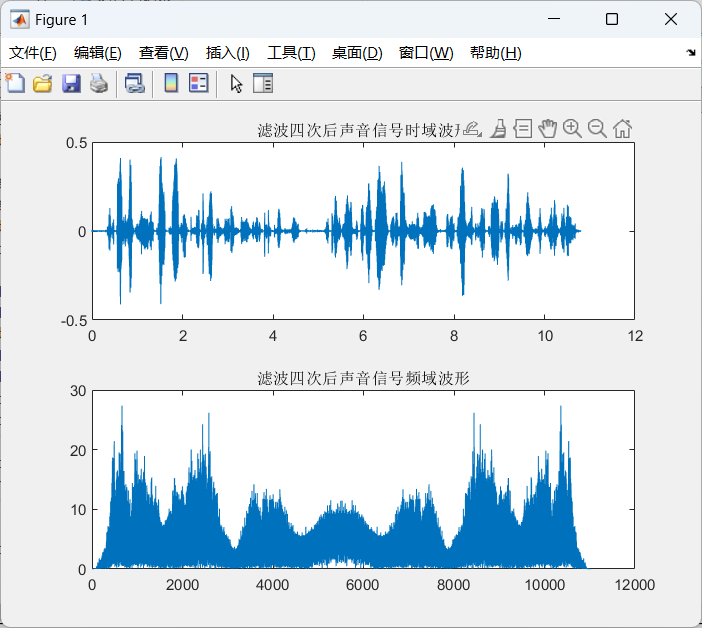
\includegraphics[width=0.6\textwidth]{5.png}
    \caption{第四次滤波后的时域频域信号}
    \label{img:5}
\end{figure}
最后就可以使用 audiowrite函数生成滤过噪音之后的音频信号保存起来。
\subsection{数字巴特沃斯带阻、高通滤波器}
同样根据原始信号的频谱制作相应的巴特沃斯带阻滤波器和高通滤波器,使用高通滤波器滤除0Hz附近的噪音,使用带阻滤波器滤除其他频率的噪音。
以下是巴特沃斯带阻滤波器代码:
\begin{verbatim}
    % butter band reject filter design
    function [afterfilter] = butter_band_reject(audio_data, f, fs)
    wp_d=f-50;
    wp_s=f+50;
    ws_d=f-150;
    ws_s=f+150;
    wp=[wp_d wp_s]*2/fs; 
    ws=[ws_d ws_s]*2/fs;
    Ap=3;As=18;
    [N,wn]=buttord(wp,ws,Ap,As);
    butter_fliter=butter(N,wn,'stop');
    afterfilter = conv(audio_data,butter_fliter);
\end{verbatim}
以下是巴特沃斯高通滤波器代码:
\begin{verbatim}
    function [afterfilter] = butter_high_pass(audio_data, f, fs)
    Ap=2;As=15;
    F_sh=f+50;
    F=2000;
    wp=F*2/fs; ws=F_sh*2/fs;
    [N,wn]=buttord(wp,ws,Ap,As);
    butter_fliter=butter(N,wn,'high');
    afterfilter = conv(audio_data,butter_fliter);
\end{verbatim}
然后主程序代码如下:
\begin{verbatim}
    % read original audio wave
    clear all;
    close all;
    [audio_data, fs] = audioread('..\dsp_lab\lab2\SunshineSquare.wav');
    time = (length(audio_data) -1)/ fs; % get audio time
    n = 0 : length(audio_data)- 1;
    tt = 0 : 1 / fs : time; % generate time vector
    % freq domain frequency resolution
    freq_res = n * fs / length(audio_data);
    audio_1 = butter_band_reject(audio_data, 1574.99, fs);
    audio_1 = audio_1(1 : end-4); % remove the last two elements.
    fft_audio_1 = fft(audio_1);
    audio_2 = butter_band_reject(audio_1, 3149.97, fs);
    audio_2 = audio_2(1 : end-4); % remove the last two elements.
    fft_audio_2 = fft(audio_2);
    audio_3 = butter_band_reject(audio_2, 4724.96, fs);
    audio_3 = audio_3(1 : end-6); % remove the last two elements.
    fft_audio_3 = fft(audio_3);
    audio_4 = butter_high_pass(audio_3, 0, fs);
    audio_4 = audio_4(1 : end-1); % remove the last two elements.
    % audio_4(abs(audio_4) > 3) = 0; % remove the pluse
    fft_audio_4 = fft(audio_4);
    subplot(2,1,1);
    plot(tt, audio_4);
    title('滤波四次后声音信号时域波形');
    subplot(2,1,2);
    plot(freq_res, abs(fft_audio_4));
    title('滤波四次后声音信号频域波形');
    soundsc(audio_4,fs);
\end{verbatim}
最终得到如图\ref{img:6}的结果
\begin{figure}[htbp]
    \centering
    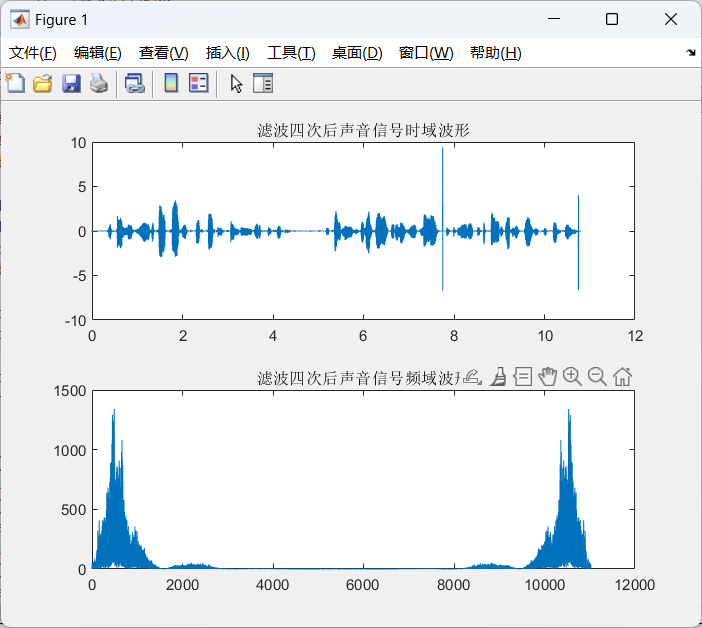
\includegraphics[width=0.6\textwidth]{6.png}
    \caption{第四次滤波后的时域频域信号}
    \label{img:6}
\end{figure}
也可以清晰地听到音频信号的内容。
但是很明显使用该滤波器滤掉噪声的同时也滤掉了部分原信号。
\section{实验小结}
本次实验,在前置实验的基础上,我用Matlab分析了音频信号的频谱,使用两种方法滤掉了音频信号中的干扰分量,第一次直观的感受到了数字滤波器的作用效果。
\end{document}